\documentclass[a4paper]{book}

% XeLaTeX: Unicode font support
\usepackage{fontspec}
\usepackage{microtype}
\microtypesetup{protrusion=true, tracking=true, final}
\clubpenalty=10000
\widowpenalty=10000
\displaywidowpenalty=10000
\tolerance=500
\emergencystretch=3em
\sloppy
\setlength{\parskip}{0.75em}
% WINDOWS %
% \setmainfont{Georgia} 
% \newfontfamily\emojifont{Segoe UI Emoji}
% UBUNTU %
\setmainfont{EB Garamond} 
\newfontfamily\emojifont{Noto Color Emoji}
\usepackage{newunicodechar}
\newunicodechar{🌓}{{\emojifont 🌓}} 
\newunicodechar{🕯}{{\emojifont 🕯}}  
\newunicodechar{️}{{\emojifont ️}}   
\newunicodechar{🙃}{{\emojifont 🙃}} % U+1F703
\newunicodechar{🌌}{{\emojifont 🌌}} % U+1F30C
\newunicodechar{🌫}{{\emojifont 🌫}} % U+1F32B
\newunicodechar{🌠}{{\emojifont 🌠}} % U+1F320
\newunicodechar{🌑}{{\emojifont 🌑}} % U+1F311
\newunicodechar{🗯}{{\emojifont 🗯}} % U+1F5EF
\newunicodechar{🌙}{{\emojifont 🌙}} % U+1F319
\newunicodechar{📯}{{\emojifont 📯}} % U+1F4EF
\newunicodechar{🙇}{{\emojifont 🙇}} % U+1F703
\usepackage[french]{babel}
\usepackage{graphicx}
\usepackage{tikz}
\usepackage[absolute,overlay]{textpos}
\usepackage{geometry}
\geometry{margin=2.5cm}
\usepackage{fancyhdr}
\pagestyle{fancy}
\fancyhead[LE,RO]{Umbranexus}
\fancyfoot[CE,CO]{\thepage}
\fancyfoot[LE,RO]{Socle Commun}
\usepackage{titlesec}
\usepackage{setspace}
\onehalfspacing
\usepackage{hyperref}
\hypersetup{colorlinks=true, linkcolor=blue, urlcolor=blue}


\providecommand{\tightlist}{
  \setlength{\itemsep}{0pt}\setlength{\parskip}{0pt}}

\usepackage{anyfontsize}
\usepackage{titlesec}
\usepackage{background}

\backgroundsetup{
  scale=1,
  color=black,
  opacity=0.3,
  angle=0,
%   position=current page.south west,
  vshift=0pt,
  hshift=0pt,
  contents={%
    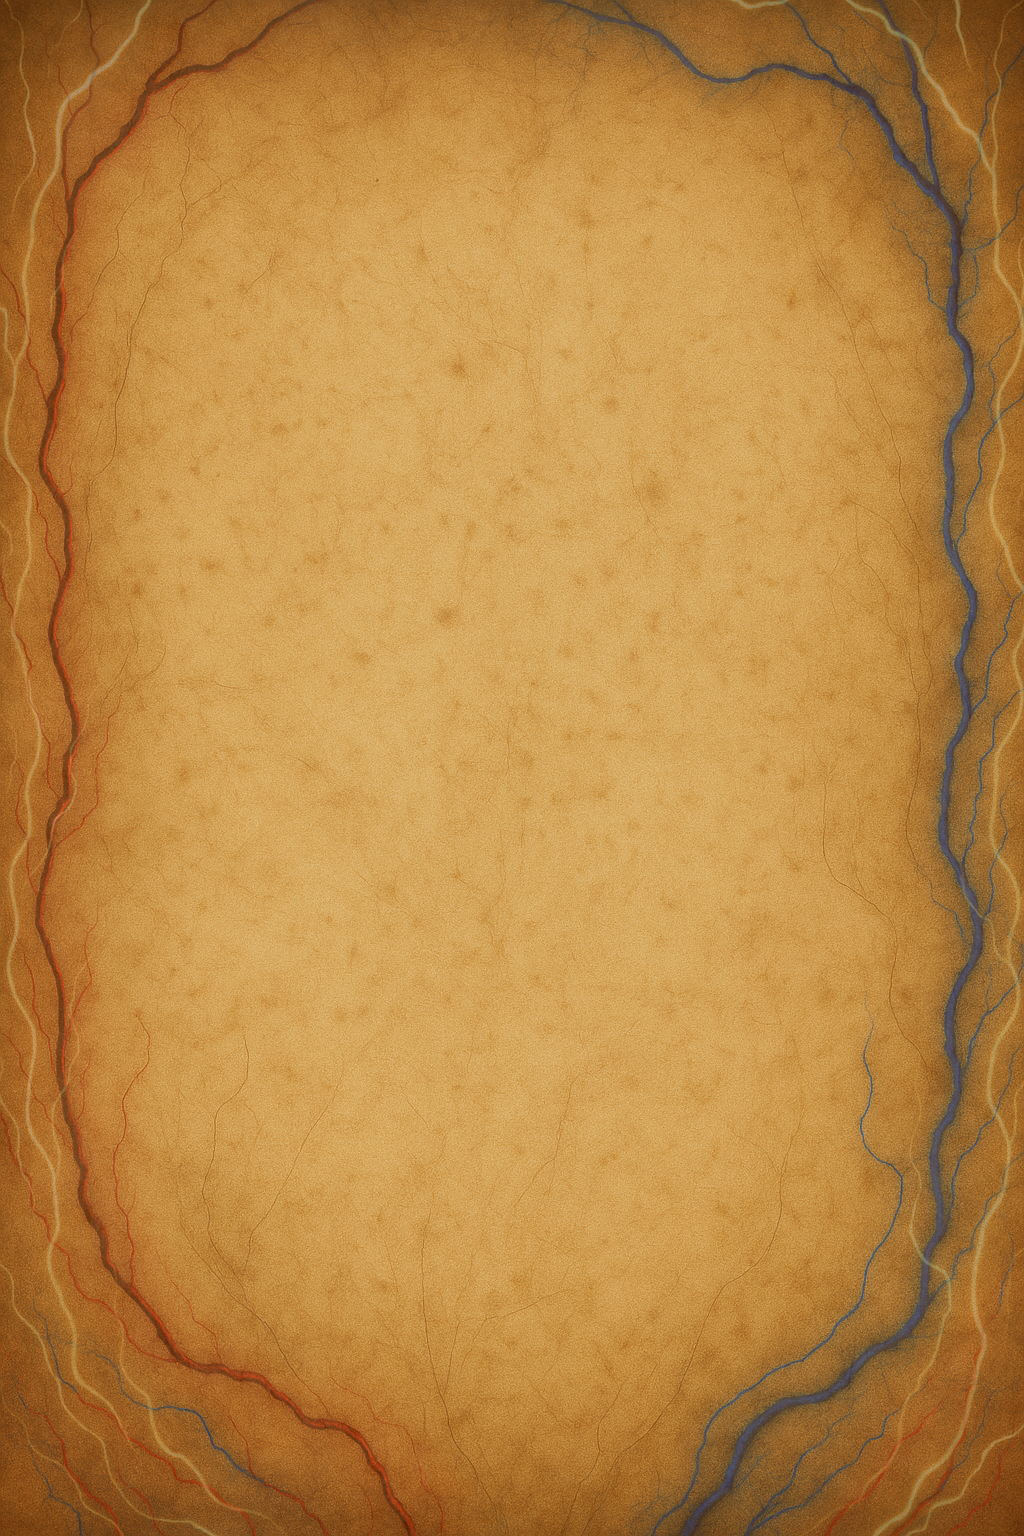
\includegraphics[width=\paperwidth,height=\paperheight]{scripts/background.png}
  }
}

\begin{document}

% COVER %
\thispagestyle{empty}
\begin{tikzpicture}[remember picture, overlay]
  \node[anchor=north west, inner sep=0pt] at (current page.north west) {
    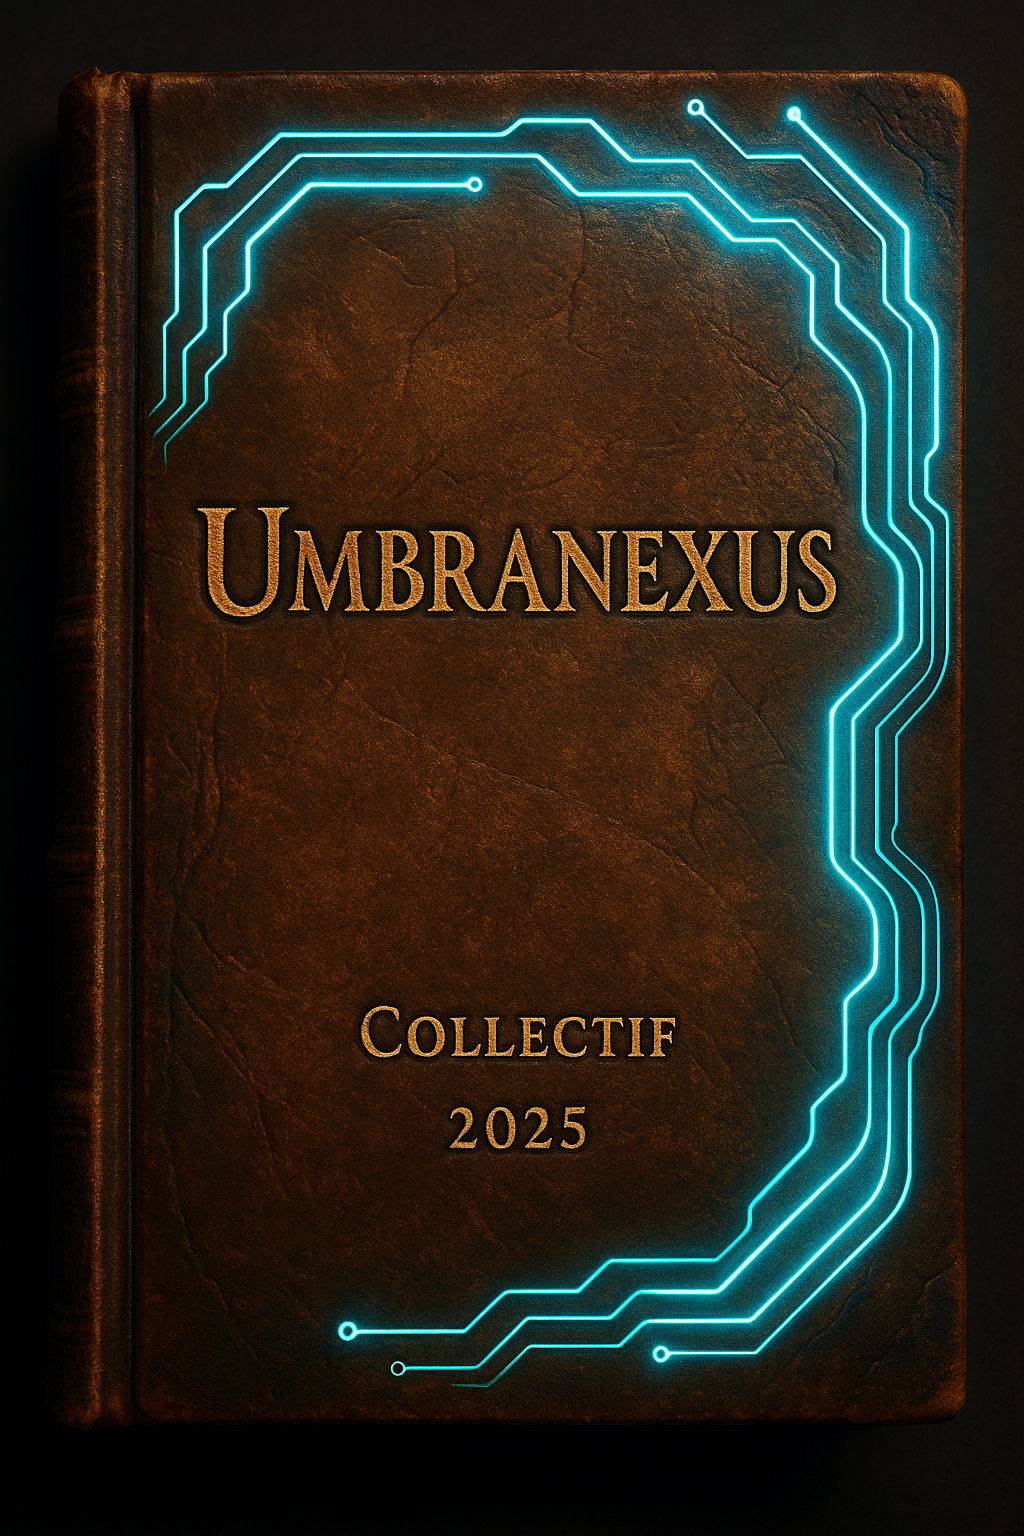
\includegraphics[width=\paperwidth,height=\paperheight]{scripts/cover.png}
  };
\end{tikzpicture}
\newpage

\thispagestyle{empty}
\vspace*{\fill}
\begin{center}
  \Large\textit{« Ce n’est pas dans la lumière que naît l’imagination,\\ mais dans l’ombre qu’elle apprivoise. »}
\end{center}
\vspace*{\fill}
\newpage

\fontsize{14pt}{16pt}\selectfont
\setcounter{secnumdepth}{-1}

% TOC %

% \cleardoublepage
% \phantomsection
% \pdfbookmark[1]{Table des matières}{toc}
% \tableofcontents
% \thispagestyle{empty}
% \newpage

% BOOK %

\renewcommand{\baselinestretch}{1.4} % Augmente l'interligne (1.4 recommandé pour la lecture)
\setlength{\parskip}{1em} % Espace entre les paragraphes
\setlength{\parindent}{0pt} % Supprime l'indentation de début de paragraphe

% \renewcommand{\thechapter}{\Roman{chapter}}

\titleformat{\chapter}[display]
  {\normalfont\bfseries\Huge}
  {}
  {0pt}
  {\Huge}
  [\vspace{1cm}]

\titleformat{\section}
  {\normalfont\Large\bfseries}
  {}{0pt}{}

\titleformat{\subsection}
  {\normalfont\large\bfseries}
  {}{0pt}{}

\titleformat{\subsubsection}
  {\normalfont\normalsize\bfseries\itshape}
  {}{0pt}{}

\titlespacing*{\section}{0pt}{1.5em}{1em}
\titlespacing*{\subsection}{0pt}{1.2em}{0.8em}
\titlespacing*{\subsubsection}{0pt}{1em}{0.5em}

$body$

\end{document}
